\chapter{Experiment and Demo}
\label{Ch-6:Sec:Experiment}
In this chapter, we will give four scenarios to describe how SEEKER works. Here is the link of \href{https://youtu.be/oog_x8N7mC4}{a two-minute demo video} on Youtube.

\section{Scenario 1: Keyword Matching}
\begin{figure*}[!htb]
	\centering
	\begin{subfigure}{0.31\textwidth}
		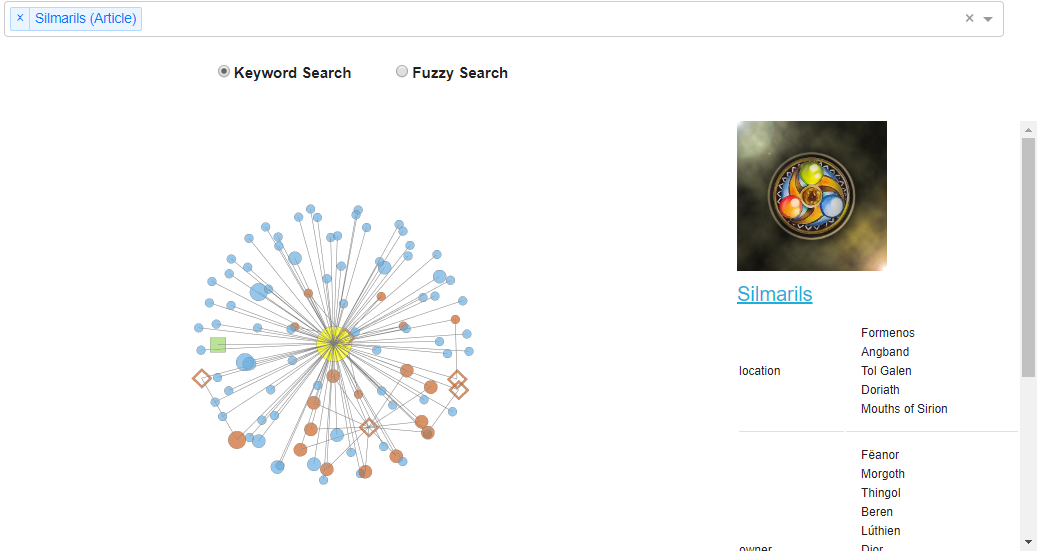
\includegraphics[width=\linewidth]{fig/Section6-1.png}
		\caption{Initialization} 
		\label{fig:section6-pic1}
	\end{subfigure}
	\hspace*{\fill} % separation between the subfigures
	\begin{subfigure}{0.31\textwidth}
		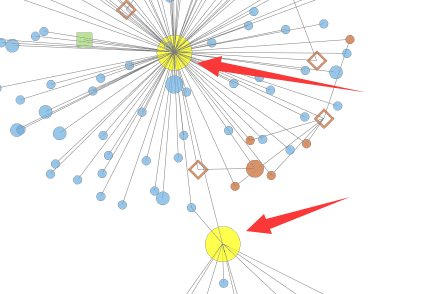
\includegraphics[width=\linewidth]{fig/Section6-2.png}
		\caption{Article Keywords} \label{fig:section6-pic2}
	\end{subfigure}
	\hspace*{\fill} % separation between the subfigures
	\begin{subfigure}{0.31\textwidth}
		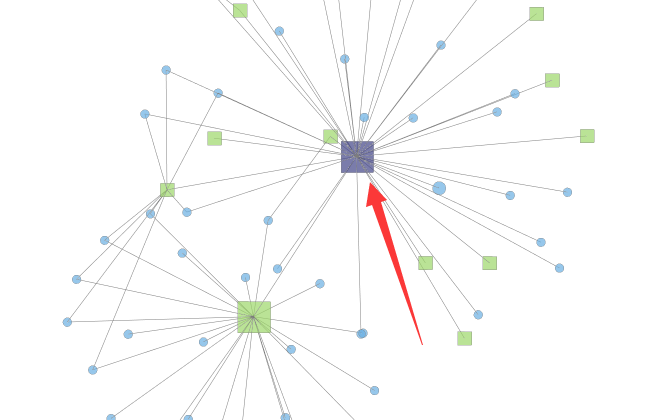
\includegraphics[width=\linewidth]{fig/Section6-3.png}
		\caption{Label Keywords} \label{fig:section6-pic3}
	\end{subfigure}
	\vspace{10pt}
	\begin{subfigure}{0.31\textwidth}
		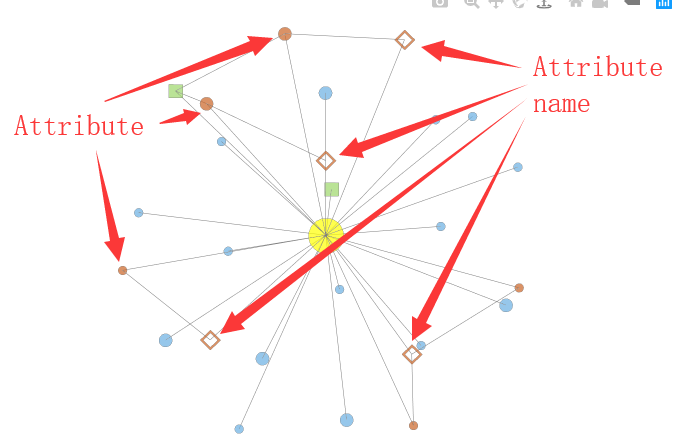
\includegraphics[width=\linewidth]{fig/Section6-4.png}
		\caption{Attributes with their names} 
		\label{fig:section6-pic4}
	\end{subfigure}
	\hspace*{\fill} % separation between the subfigures
	\begin{subfigure}{0.31\textwidth}
		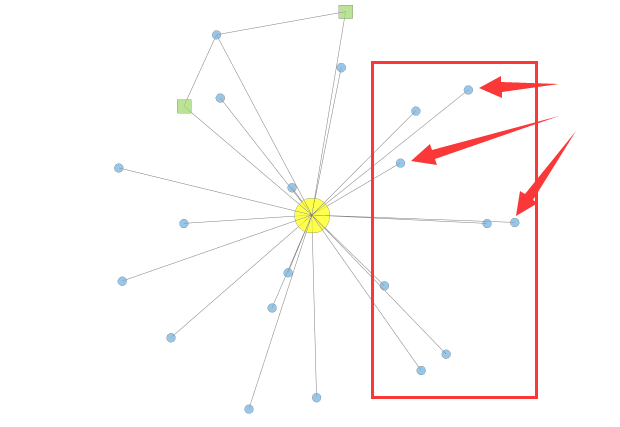
\includegraphics[width=\linewidth]{fig/Section6-5.png}
		\caption{Neighbors} \label{fig:section6-pic5}
	\end{subfigure}
	\hspace*{\fill} % separation between the subfigures
	\begin{subfigure}{0.31\textwidth}
		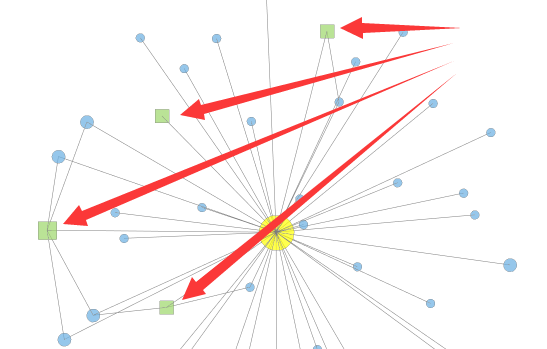
\includegraphics[width=\linewidth]{fig/Section6-6.png}
		\caption{Labels of keywords} \label{fig:section6-pic6}
	\end{subfigure}
	\vspace{-10pt}
	\caption{Scenario 1: Keyword Matching} \label{fig:section6-pic234}
\end{figure*}
\vspace{-10pt}
In Figure~\ref{fig:section6-pic234}, we can see the initialization of SEEKER (Figure~\ref{fig:section6-pic1}). The yellow circles represent article keywords (Figure~\ref{fig:section6-pic2}), while purple squares represent label keywords (Figure~\ref{fig:section6-pic3}). Red circles are attributes, which connected to their red square-frame attribute names (Figure~\ref{fig:section6-pic4}) and blue circles are neighbors of keywords (Figure~\ref{fig:section6-pic5}). Green squares illustrate the labels of keywords (Figure~\ref{fig:section6-pic6}). The size of those shapes shows their importance to the keywords.

\section{Scenario 2: Finding Relationships}
\begin{figure*}[!htb]
	\centering
	\begin{subfigure}{0.31\textwidth}
		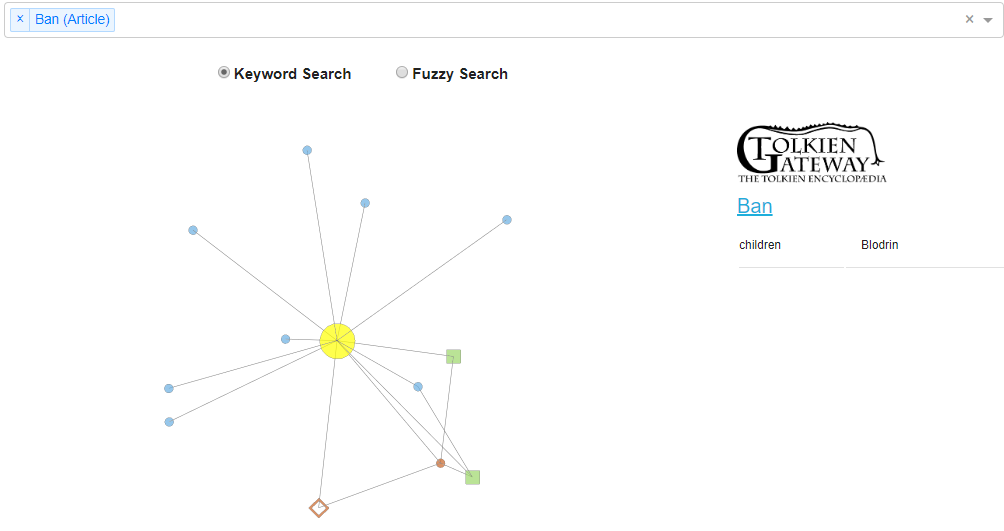
\includegraphics[width=\linewidth]{fig/Section6-7.png}
		\caption{Initialization} 
		\label{fig:section6-pic7}
	\end{subfigure}
	\hspace*{\fill} % separation between the subfigures
	\begin{subfigure}{0.31\textwidth}
		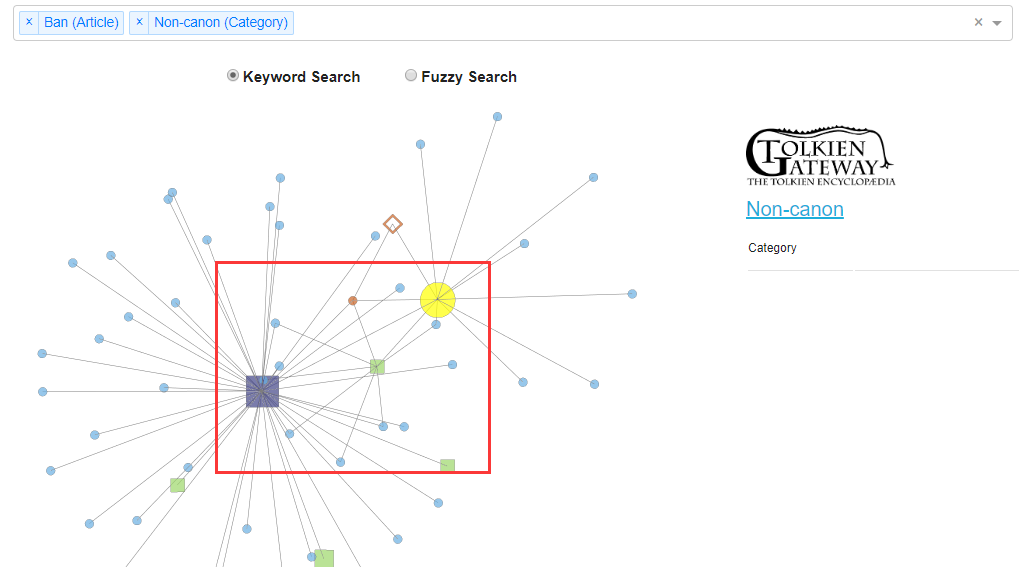
\includegraphics[width=\linewidth]{fig/Section6-8.png}
		\caption{Click a square} \label{fig:section6-pic8}
	\end{subfigure}
	\hspace*{\fill} % separation between the subfigures
	\begin{subfigure}{0.31\textwidth}
		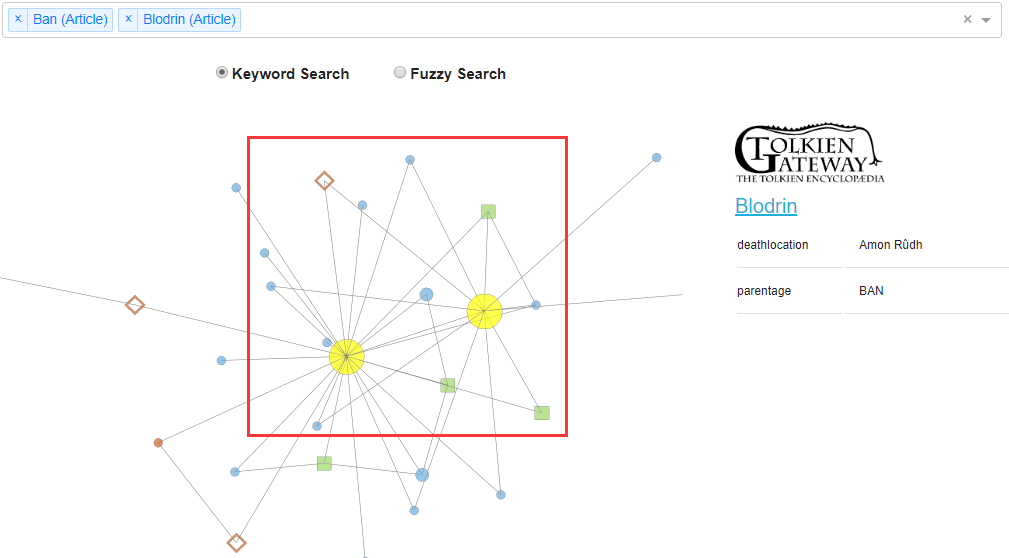
\includegraphics[width=\linewidth]{fig/Section6-9.png}
		\caption{Click a circle} \label{fig:section6-pic9}
	\end{subfigure}
	\vspace{10pt}
	\begin{subfigure}{0.31\textwidth}
		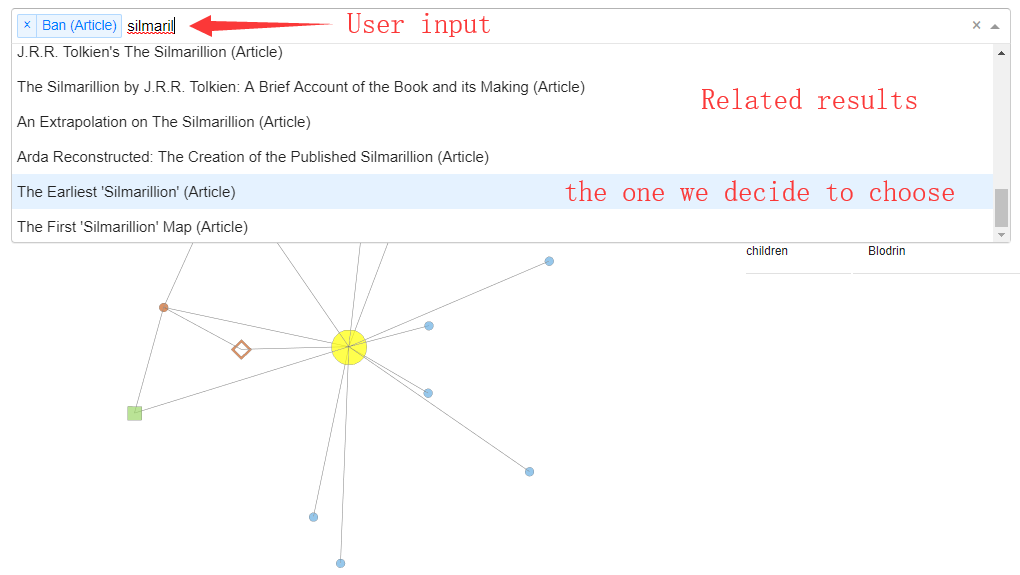
\includegraphics[width=\linewidth]{fig/Section6-10.png}
		\caption{Input a word} 
		\label{fig:section6-pic10}
	\end{subfigure}
	\hspace*{\fill} % separation between the subfigures
	\begin{subfigure}{0.31\textwidth}
		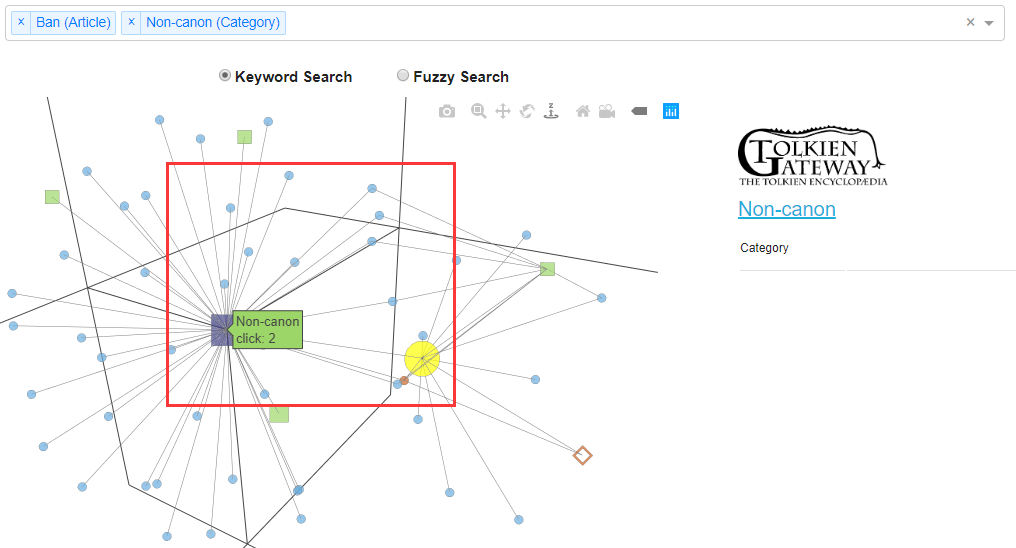
\includegraphics[width=\linewidth]{fig/Section6-12.png}
		\caption{Choose a label keyword} \label{fig:section6-pic11}
	\end{subfigure}
	\hspace*{\fill} % separation between the subfigures
	\begin{subfigure}{0.31\textwidth}
		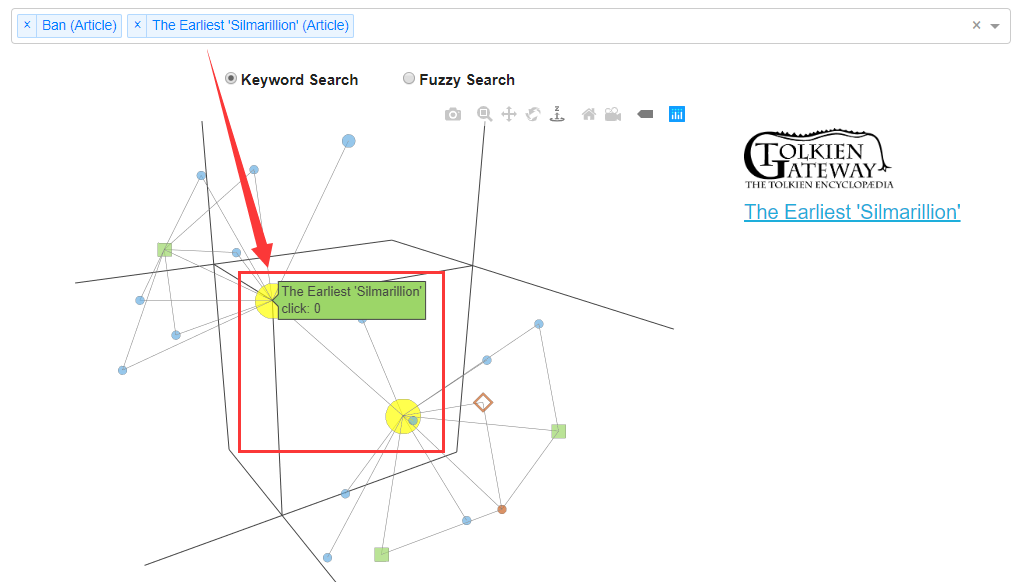
\includegraphics[width=\linewidth]{fig/Section6-11.png}
		\caption{Select an article keyword} \label{fig:section6-pic12}
	\end{subfigure}
	\vspace{-10pt}
	\caption{Scenario 2: Find Relationships} \label{fig:section6-pic789}
	\vspace{-20pt}
\end{figure*}
\vspace{-25pt}
In scenario 2, we will introduce two ways to find the relationships between keywords.\\
The first way is clicking a linked green square (label) (Figure~\ref{fig:section6-pic8}) or a blue circle (article) (Figure~\ref{fig:section6-pic9}).
The second way is using the input box. Users can input what they want to find and the program will help them find the similar keyword (Figure~\ref{fig:section6-pic10}). We can see the edges and nodes inside the red frame are the relationships between keywords in the input box (Figure~\ref{fig:section6-pic11} and \ref{fig:section6-pic12}).

\section{Scenario 3: User Feedback Enhancement}
\begin{figure*}[!htb]
	\centering
	\begin{subfigure}{0.47\textwidth}
		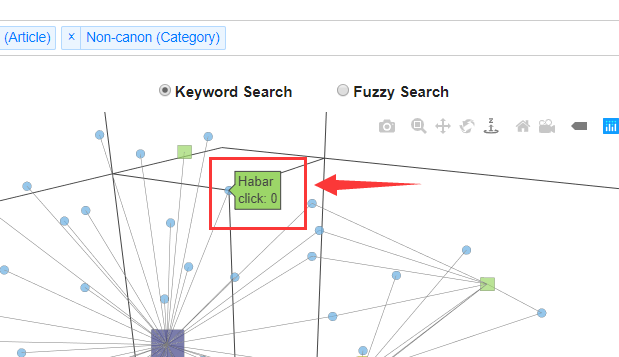
\includegraphics[width=\linewidth]{fig/Section6-13.png}
		\caption{Before click an article node} 
		\label{fig:section6-pic13}
	\end{subfigure}
	\hspace*{\fill} % separation between the subfigures
	\begin{subfigure}{0.47\textwidth}
		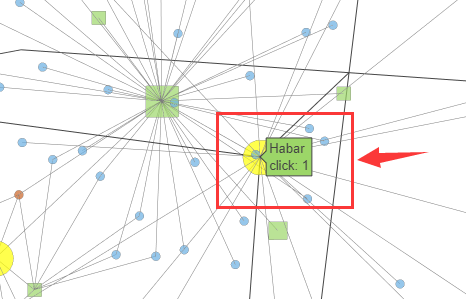
\includegraphics[width=\linewidth]{fig/Section6-14.png}
		\caption{After click an article node} \label{fig:section6-pic14}
	\end{subfigure}
	\vspace{10pt}
	\begin{subfigure}{0.47\textwidth}
		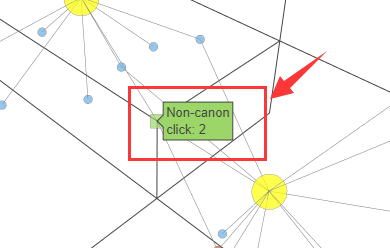
\includegraphics[width=\linewidth]{fig/Section6-15.png}
		\caption{Before click a label} \label{fig:section6-pic15}
	\end{subfigure}
	\hspace*{\fill} % separation between the subfigures
	\begin{subfigure}{0.47\textwidth}
		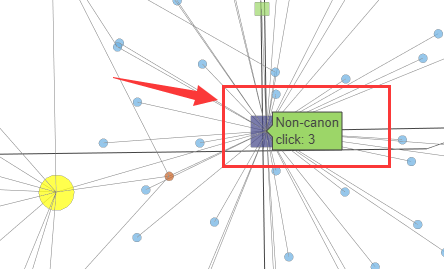
\includegraphics[width=\linewidth]{fig/Section6-16.png}
		\caption{After click a label} 
		\label{fig:section6-pic16}
	\end{subfigure}
	\vspace{-10pt}
	\caption{Scenario 3: User Feedback Enhancement} \label{fig:section6-pic101112}
\end{figure*}
\vspace{-25pt}
The user feed back enhancement works when SEEKER plots the graph and users click the circles and squares.\\
\indent There is a file which records the action of user click events. Every time the user clicks on the node, the click times of that node will plus 1. What's more, the click times is added to the size of node. If the user clicks one node for several times, the size will increase until it reaches the upper bound.\\
\indent In Figure~\ref{fig:section6-pic13}, we can see the click times of ``Habar'' is 0. After the user clicks that blue node, it becomes a keyword (larger yellow circle) and the click times increases to 1 (Figure~ \ref{fig:section6-pic14}). In Figure~\ref{fig:section6-pic15}, the click times of ``Non-conon'' is 2. After clicking, it becomes a keyword (larger purple square) and the click times raises to 3 (Figure~\ref{fig:section6-pic16}).

\section{Scenario 4: Answering Natural Language Questions}
\begin{figure*}[!htb]
	\centering
	\begin{subfigure}{0.47\textwidth}
		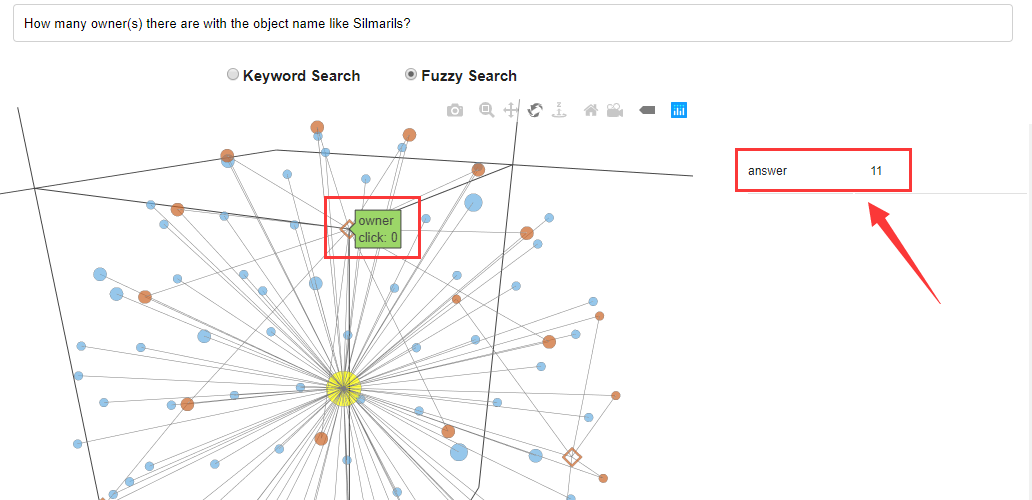
\includegraphics[width=\linewidth]{fig/Section6-17.png}
		\caption{Fuzzy Search} 
		\label{fig:section6-pic17}
	\end{subfigure}
	\hspace*{\fill} % separation between the subfigures
	\begin{subfigure}{0.47\textwidth}
		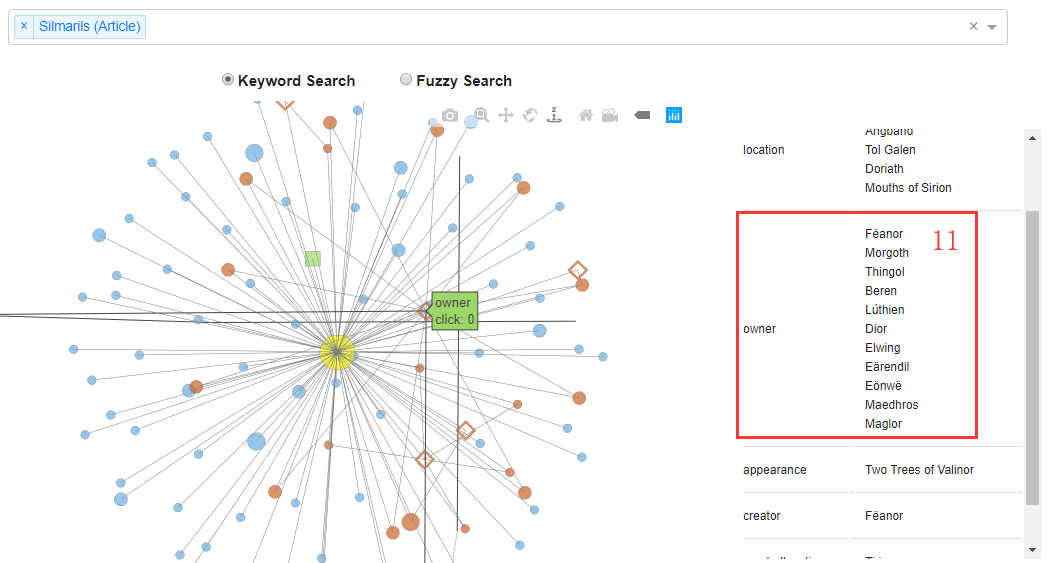
\includegraphics[width=\linewidth]{fig/Section6-18.png}
		\caption{Using keyword search to verify results} \label{fig:section6-pic18}
	\end{subfigure}
	\vspace{-10pt}
	\caption{Scenario 4: Answering Natural Language Questions} \label{fig:section6-pic1718}
	\vspace{-20pt}
\end{figure*}
\vspace{-30pt}
In this scenario, we will test the natural language processing part. The user asks a question ``How many owner(s) there are with the object name like Silmarils?''. Then, SEEKER can give the answer of this question as ``11'' on right side of the screen (Figure~\ref{fig:section6-pic17}). Thus, users can get the information directly and don't need to count the names one by one.\\
\indent Finally, we use the keyword search to verify the result. In Figure~ \ref{fig:section6-pic18}, we can see that the 11 owners of Silmarils are Fëanor, Morgoth, Thingol, Beren, Lúthien, Dior, Elwing, Eärendil, Eönwë, Maedhros and Maglor. Thus, the answer of Fuzzy Search is correct.
